\documentclass[10pt,oneside]{book} %oneside es para eliminar las hojas en blanco entre cada capítulo
\usepackage[pdftex]{graphicx}
% letterpaper
\usepackage[utf8]{inputenc}
\usepackage[spanish]{babel} % varias definiciones para el español (por ejemplo usa ''Índice'' en lugar de ''Contents'')
\usepackage{hyperref}
\usepackage{geometry}
\usepackage{multicol}
%Para mostrar c\'odigo fuente
\usepackage{listings}
% Libraries for diagrams
\usepackage{tikz}
\usetikzlibrary{shapes,arrows}
\usepackage{caption}
%%%%%%%%%%%%%%%%%%%%%%%%%%%%%

\lstset
{%
        %linewidth=\linewidth,  
        breaklines=true,
        tabsize=1, 
        showstringspaces=false%      
}
%\usepackage{lstautogobble}
%
\usepackage{mdwlist}
%\usepackage{enumitem}
%\usepackage{ragged2e}
%\addcontentsline{toc}{itemize}{Lista de informaci\'on}
\geometry{
    a5paper,
%     a6paper,
%     total={210mm,297mm},
    left=20mm,
    right=20mm,
    top=20mm,
    bottom=20mm,
    bindingoffset=0mm
}
\title{T\'itulo del libro}
\author{Jorge Bautista}


\begin{document}
    \frontmatter
    \maketitle
    %Prólogo del libro
    
\chapter{Pr\'ologo}
Este es un libro que menciona de manera breve todas las caracter\'isticas del framework \href{``http://www.grails.org/''}{'Grails'} descritas en el libro \textit{``The Definitive Guide To Grails''}. No se detiene a explicar detalles. Simplemente permite que el lector se asome a la tecnolog\'ia para comenzar a conocerla o para buscar posibles soluciones a problemas encontrados durante el desarrollo.


    
    \mainmatter
    %Cap\'itulo 1: 'B\'asicos'
    % \chapter{Arquitectura y comandos b\'asicos}
\chapter{Arquitectura de grails}
Grails envuelve a muchas tecnolog\'ias relacionados con \textit{java}, abstrayendo su complejidad al proporcionarnos configuraciones predeterminadas que cubren los casos de uso m\'as comunes. Estas configuraciones pueden ahorrarnos d\'ias o semanas de trabajo debido a la integraci\'on con otras tecnolog\'ias.

Aqu\'i se presentan las tecnolog\'ias principales sobre las que se Grails est\'a montado:
%En este cap\'itulo se listan las tecnolog\'ias que usa grails y comandos b\'asicos para comenzar a usarlo. 

\begin{multicols}{2}
\begin{itemize}
  \item Hibernate
  \item Spring
  \item Sitemesh
  \item Tomcat
  \item H2
  \item Groovy
  \item Gant
  \item JEE
\end{itemize}
\end{multicols}

\begin{figure}[ht!]

    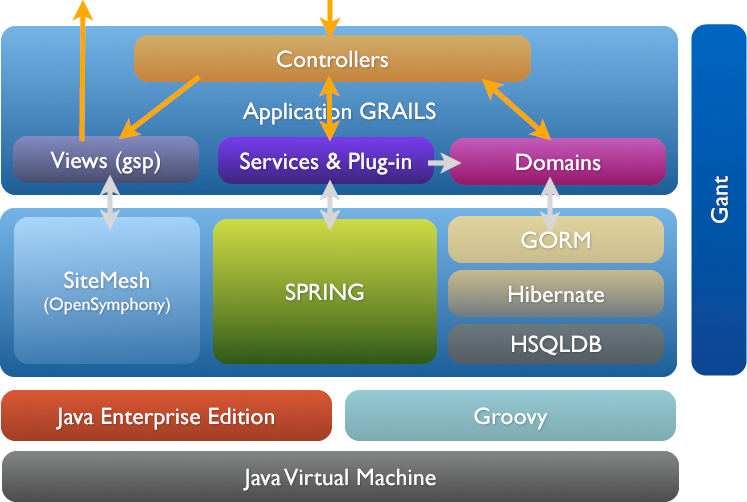
\includegraphics[width=100mm]{img/arch}
    \caption{Tecnolog\'ias que confirman la arquitectura de Grails}
    \label{arquitectura}
    

\end{figure}


    % \chapter{Arquitectura y comandos b\'asicos}
\chapter{M\'etodos de renderizado}

% Define block styles
\tikzstyle{decision} = [diamond, draw, fill=blue!20, 
    text width=4.5em, text badly centered, node distance=3cm, inner sep=0pt]
\tikzstyle{block} = [rectangle, draw, fill=blue!20, 
    text width=5em, text centered, rounded corners, minimum height=4em]
\tikzstyle{line} = [draw, -latex']
\tikzstyle{cloud} = [draw, ellipse,fill=white, node distance=3cm,
    minimum height=2em]

    
\begin{figure}[ht!]
    \begin{tikzpicture}[node distance = 2cm, auto]

        % Place nodes
        \node [block] (init) {controllers};
        \node [cloud, left of=init, node distance=5.1cm] (views) {views};
        \node [cloud, right of=init, node distance=3.4cm] (services) {services};    
        \node [cloud, below of=views] (views2) {views};
    %     \node [block, below of=init] (identify) {identify candidate models};
    %     \node [block, below of=identify] (evaluate) {evaluate candidate models};
    %     \node [block, left of=evaluate, node distance=3cm] (update) {update model};
    %     \node [decision, below of=evaluate] (decide) {is best candidate better?};
    %     \node [block, below of=decide, node distance=3cm] (stop) {stop};

        % Draw edges
        \path [line] (views) -- node [auto] {1.-jquery, canjs, form} (init);
    %     \path [line] (views) -- (views);
        \path [line] (init) -- node [auto] {2.-invoke} (services);
        \path [line] (init) -- node [auto] {3.-render: views, json, txt} (views2);
        
    %     \path [line] (init) -- (identify);
    %     \path [line] (identify) -- (evaluate);
    %     \path [line] (evaluate) -- (decide);
    %     \path [line] (decide) -| node [near start] {yes} (update);
    %     \path [line] (update) |- (identify);
    %     \path [line] (decide) -- node {no}(stop);
    %     \path [line,dashed] (expert) -- (init);
    %     \path [line,dashed] (system) -- (init);
    %     \path [line,dashed] (system) |- (evaluate);
    \end{tikzpicture}
    \caption{Flujo de datos b\'asico de Grails}
\end{figure}


% \begin{tikzpicture}[node distance = 2cm, auto]
%     
%     \node [block] (init) {initialize model};
%     \node [cloud, left of=init] (expert) {expert};
%     \node [cloud, right of=init] (system) {system};
%     \node [block, below of=init] (identify) {identify candidate models};
%     \node [block, below of=identify] (evaluate) {evaluate candidate models};
%     \node [block, left of=evaluate, node distance=3cm] (update) {update model};
%     \node [decision, below of=evaluate] (decide) {is best candidate better?};
%     \node [block, below of=decide, node distance=3cm] (stop) {stop};
%     
%     \path [line] (init) -- (identify);
%     \path [line] (identify) -- (evaluate);
%     \path [line] (evaluate) -- (decide);
%     \path [line] (decide) -| node [near start] {yes} (update);
%     \path [line] (update) |- (identify);
%     \path [line] (decide) -- node {no}(stop);
%     \path [line,dashed] (expert) -- (init);
%     \path [line,dashed] (system) -- (init);
%     \path [line,dashed] (system) |- (evaluate);
% \end{tikzpicture}
El resultado enviado de los controllers a las vistas puede ir en varios formatos. Siempre se hace a trav\'es de la instrucci\'ion \textit{render}:
\begin{itemize}

    \item \textbf{Renderizar texto}    
        \begin{lstlisting}[gobble=11] 
            render 'Welcome to the gTunes store!'
        \end{lstlisting}

    \item \textbf{Solicitar ayuda de un comando}
        \begin{lstlisting}[gobble=11]
            grails help NOMBRE_DE_COMANDO
        \end{lstlisting}

    \item \textbf{Crear aplicaci\'on de Grails}
        \begin{lstlisting}[gobble=11]
            grails create-app NOMBRE_DE_APP
        \end{lstlisting}


    \item \textbf{Crear un controller + sus pruebas + sus vistas}
        \begin{lstlisting}[gobble=11]
            grails create-controller [PAQUETE]NOMBRE
        \end{lstlisting}

    \item \textbf{Ejecutar pruebas de la aplicaci\'on}
        \begin{lstlisting}[gobble=11]
            grails test-app
        \end{lstlisting}

    \item \textbf{Ejecutar la aplicaci\'on}
        \begin{lstlisting}[gobble=11]
            grails run-app
        \end{lstlisting}
        
\end{itemize}

%     \backmatter
    \appendix    
    % \chapter{Arquitectura y comandos b\'asicos}
\chapter{Comandos m\'as comunes}

\begin{itemize}

    \item \textbf{Consultar versi\'on de Grails}    
        \begin{lstlisting}[gobble=11] 
            grails -version
        \end{lstlisting}
        Devolver\'a una l\'inea de texto describiendo la versi\'on de grails.

    \item \textbf{Solicitar ayuda de un comando}
        \begin{lstlisting}[gobble=11]
            grails help NOMBRE_DE_COMANDO
        \end{lstlisting}
        Devolver\'a informaci\'on (no tan detallada) sobre el comando y sus argumentos.

    \item \textbf{Crear aplicaci\'on de Grails}
        \begin{lstlisting}[gobble=11]
            grails create-app NOMBRE_DE_APP
        \end{lstlisting}
        Genera toda la estructura de archivos de una aplicaci\'on de Grails.

    \item \textbf{Crear un controller + sus pruebas + sus vistas}
        \begin{lstlisting}[gobble=11]
            grails create-controller [PAQUETE]NOMBRE
        \end{lstlisting}
        Genera un controlador de Grails as\'i como archivos de prueba y \textit{gsp's}. Tanto los archivos de prueba como los \textit{gsp's} se generan vac\'ios.

    \item \textbf{Ejecutar pruebas de la aplicaci\'on}
        \begin{lstlisting}[gobble=11]
            grails test-app
        \end{lstlisting}
        Ejecuta todas las pruebas de la aplicaci\'on, poniendo los resultados en \textit{test/reports}

    \item \textbf{Ejecutar la aplicaci\'on}
        \begin{lstlisting}[gobble=11]
            grails [ENVIRONMENT] run-app
        \end{lstlisting}
        Ejecuta la aplicaci\'on. Si ENVIRONMENT no se especifica, el default a usar ser\'a el de desarrollo (development).
        
    \item \textbf{Crear clase de dominio}
        \begin{lstlisting}[gobble=11]
            grails create-domain-class [PAQUETE]NOMBRE
        \end{lstlisting}        
        Se encarga de crear una nueva clase de dominio y adem\'as genera un archivo donde pueden implantarse sus pruebas.
\end{itemize}

    
    \listoffigures
    \listoftables
    %\nocite{*}
    \begin{thebibliography}{99}    
        \bibitem{bib-name1} article-description1
        \bibitem{bib-name2} article-description2
    \end{thebibliography}
\end{document}

%\documentclass[a4paper,10pt]{book}
%\usepackage[utf8]{inputenc}

%\begin{document}

%\end{document}
